% Student Number: 2240357068
% Student Name: Baturay KAFKAS
% EEE @ Hacettepe University

% My resource collection: https://github.com/kfksbtry/uni
% Circuits were set up in LTspice.

\documentclass{article}

\usepackage{graphicx}
\usepackage[top=25mm, bottom=25mm, left=25mm, right=25mm]{geometry}
\usepackage{amsmath}
\usepackage{moresize}
\usepackage{parskip}
\usepackage{float}
\usepackage{fancyhdr}
\usepackage{booktabs}
\usepackage{pgfplots}
\pgfplotsset{compat=1.18}
\usepackage{tikz}

\pagestyle{fancy}
\fancyhf{}
\fancyhead[R]{Baturay KAFKAS 2240357068 Electrical \& Electronics Engineering}

\rfoot{\thepage}
\renewcommand{\headrulewidth}{0pt} 
\renewcommand{\footrulewidth}{0pt}

\begin{document}

\large
\textit{This part of the experiment is prepared with Online LaTeX Editor Overleaf. Visit the website for the source here:}

\textbf{https://www.overleaf.com/read/hwfqkkbqkbns\#9a3ac6}

\hrule

\vspace{1em}

\textbf{1. EXPERIMENT 4 - PRELIMINARY WORK}

\textbf{1.1} For the circuit given in \textit{Fig. 1}, sketch roughly the waveforms of $V_L(t)$ and $V_R(t)$.

\begin{figure}[H]
    \centering
    \includegraphics[width=0.75\linewidth]{chrome_mGt3fLR2f2.png}
\end{figure}

\textbf{Answer}: Let $I_S$ be the current in the circuit. Use a KVL equation for $0<t<1.8$ ms.

\[V_S-V_R-V_L=0\implies V_S=120I_S+36\times10^{-3}\,\dfrac{dI_S}{dt}\implies\dfrac{V_S-120I_S}{36\times10^{-3}}=\dfrac{dI_S}{dt}\]

Rearrange the equation.

\[\dfrac{10^3}{36}\,dt=\frac{dI_S}{V_S-120I_S}\implies\frac{10^3}{36}\int_0^{t}d\tau=\int_{I_S(0)}^{I_S(t)}\frac{dx}{V_S-120x}\]

\[\implies\left.\frac{10^3\tau}{36}\right|_{\tau=0}^{\tau=t}=\left.-\frac{1}{120}\ln\left|V_S-120x\right|\right|_{x=I_S(0)}^{x=I_S(t)}\implies-\frac{250t}9=\frac1{120}\ln\left(\frac{V_S-120I_S(t)}{V_S-120I_S(0)}\right)\]

\[\implies e^{-10000t/3}=\frac{V_S-120I_S(t)}{V_S-120I_S(0)}\implies I_S(t)=\frac{V_S}{120}+\left(I_S(0)-\frac{V_S}{120}\right)e^{-10000t/3}\]

The current in the circuit decays exponentially over time. The voltages across the inductor and the resistor, respectively, are

\[V_L=L\frac{dI_S}{dt}=36\times10^{-3}\cdot\left(I_S(0)-\frac{V_S}{120}\right)e^{-10000t/3}\cdot\left(-\frac{10000}3\right)=(V_S-120I_S(0))e^{-10000t/3}\]

\[V_R=I_SR=V_S+\left(120I_S(0)-V_S\right)e^{-10000t/3}\]

One problem is that we need to know the value of $I_S(0)$, which is not given in the question. Let's assume that $I_S=-\dfrac{V_S(0^+)}{120}$, then

\[\left.\begin{array}{l}
V_L(t)=10e^{-10000t/3}\text{ V}\\
V_R(t)=5-10e^{-10000t/3}\text{ V}
\end{array}\right\}\:0< t< 1.8\text{ ms}\]

For $1.8\text{ ms}< t<3.6\text{ ms}$, the polarity of the source changes. Assume that the final voltages are attained, i.e., the difference in the voltage at $t=1.8$ ms and the final voltage is negligible. Therefore, the equations also change sign.

\[\left.\begin{array}{l}
V_L(t)=-10e^{-10000(t-1.8\text{ ms})/3}\text{ V}\\
V_R(t)=-5+10e^{-10000(t-1.8\text{ ms})/3}\text{ V}
\end{array}\right\}\:1.8\text{ ms}< t< 3.6\text{ ms}\]

Since $0< t<3.6\text{ ms}$ comprises one square wave, we can sketch the entire graph.

\begin{center}
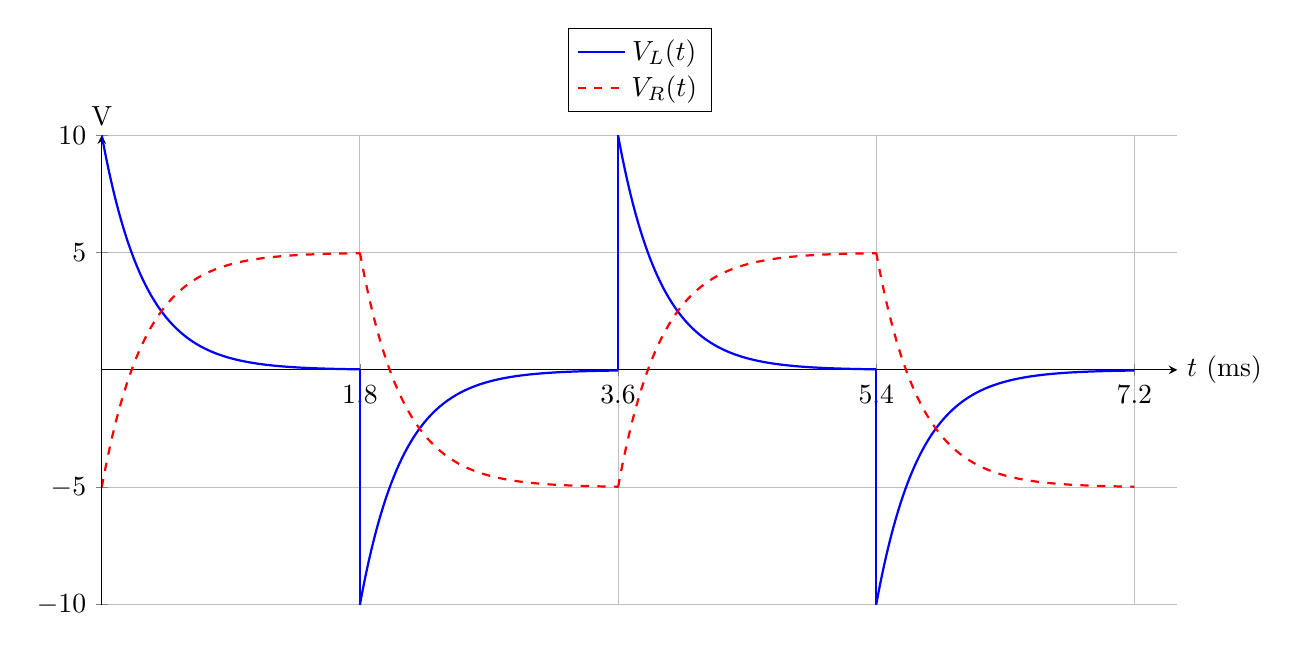
\begin{tikzpicture}
\begin{axis}[
    axis lines=center,
    width=14cm,
    height=7cm,
    xlabel={$t$ (ms)}, ylabel={V},
    xlabel style={at={(axis description cs:1,0.5)}, anchor=west}, % right end
    ylabel style={at={(axis description cs:0,1)}, anchor=south}, % above
    grid=both,
    xmin=0, xmax=7.5,
    domain=0:7.2,
    samples=300,
    legend style={at={(0.5,1.05)},anchor=south},
    scale=1.1,
    xtick={1.8,3.6,5.4,7.2}
]

\addlegendimage{blue, thick}
\addlegendentry{$V_L(t)$}

\addlegendimage{red, thick, dashed}
\addlegendentry{$V_R(t)$}

% V_L(t)
\addplot[blue, thick, domain=0:1.8, forget plot] {10*exp(-10*x/3)};
\addplot[blue, thick, domain=1.8:3.6, forget plot] {-10*exp(-10*(x-1.8)/3)};
\addplot[blue, thick, domain=3.6:5.4, forget plot] {10*exp(-10*(x-3.6)/3)};
\addplot[blue, thick, domain=5.4:7.2, forget plot] {-10*exp(-10*(x-5.4)/3)};

% V_R(t) 
\addplot[red, thick, dashed, domain=0:1.8, forget plot] {5 - 10*exp(-10*x/3)};
\addplot[red, thick, dashed, domain=1.8:3.6, forget plot] {-5 + 10*exp(-10*(x-1.8)/3)};
\addplot[red, thick, dashed, domain=3.6:5.4, forget plot] {5 - 10*exp(-10*(x-3.6)/3)};
\addplot[red, thick, dashed, domain=5.4:7.2, forget plot] {-5 + 10*exp(-10*(x-5.4)/3)};

\draw[blue, thick] (axis cs:1.8,-10) -- (axis cs:1.8,0);
\draw[blue, thick] (axis cs:3.6,10) -- (axis cs:3.6,0);
\draw[blue, thick] (axis cs:5.4,-10) -- (axis cs:5.4,0);

\end{axis}
\end{tikzpicture}
\end{center}
\end{document}